\documentclass[letterpaper]{article}
\usepackage[T1]{fontenc}
\usepackage[utf8]{inputenc}
\usepackage{tocloft,siunitx,amssymb,amsmath,graphicx,float}
\usepackage[top=3cm,left=3cm,right=3cm]{geometry}
\usepackage{pgf,pgfplots}
\usepackage[american]{circuitikz}
\graphicspath{{img/}}
\renewcommand\cftsecfont{\normalfont}
\renewcommand\cftsecpagefont{\normalfont}
\renewcommand{\cftsecleader}{\cftdotfill{\cftsecdotsep}}
\renewcommand\cftsecdotsep{\cftdot}
\renewcommand\cftsubsecdotsep{\cftdot}
\renewcommand\cftsubsubsecdotsep{\cftdot}
\title{Lab 6:Nodal Analysis}
\author{
    Sebastián Nava López\\
    \and
    Ericka Sabrina Pensamiento R.\\
    \and
    Salvador Palos Gil
}
%\captionsetup[subfigure]{justification=raggedright}
\begin{document}
\begin{titlepage}
    \centering
    {\Huge Instituto Politécnico Nacional}\\[3ex]
    {\huge Escuela Superior de Cómputo}\\[8ex]
    {\huge Fundamental Circuit Analysis}\\[12ex]
    {\Large Lab 6:Nodal Analysis(DC)}\\[20ex]
    {\Large Group: 1CV5 Team: 7 \\[8ex]
    Sebastian Nava López\\[4ex]
    Sabrina Erika Pensamiento Robledo\\[4ex]
    Salvador Palos Gil\\[18ex]
    }
    \large{Elaboration: April 24, 2018 \hspace{8em} Due date: May 1, 2018}
\end{titlepage}
\tableofcontents
\newpage
\section{Introduction}
\newpage
\section{Development}
\subsection{Verification of nodal analysis in DC}
We wired a circuit as shown in the diagram in figure \ref{fig:1}
\begin{figure}[H]
    \centering
    \begin{circuitikz}[scale=0.95,transform shape]
    \draw (0,0) to [V=$V_{S1}:\SI{9}{\volt}$,invert](0,3) -- (0,5)
    to [R=$R_1:\SI{330}{\ohm}$](6,5) -- (6,3)
    to [R=$R_4:\SI{680}{\ohm}$](6,0) -- (0,0)
    (0,3) to [R=$R_2:\SI{1}{\kilo\ohm}$,*-*](3,3)
    to [V=$V_{S2}:\SI{5}{\volt}$,-*](6,3)
    (3,0) to [R=$R_3:\SI{560}{\ohm}$,*-*](3,3)
    (3,0) to node[ground]{}(3,-0.3);
    \end{circuitikz}
    \caption{Circuit diagram}
    \label{fig:1}
\end{figure}
Then, we measured voltage values in each node and currents on each resistor and voltage
source. Afterwards, we measured the voltage in each resistor so we can calculate the power values for each
component.
\subsubsection{Measurements}
First, in order to use nodal analysis to find the voltages in the nodes of our circuit, we
need to declare the circuit currents, in this case, we do it as shown in figure \ref{fig:2}
\begin{figure}[H]
    \centering
    \begin{circuitikz}[scale=0.95,transform shape]
    \draw (0,0) to [V=$V_{S1}$,invert](0,3) -- (0,5)
    to [R=$R_1$](6,5) -- (6,3)
    to [R=$R_4$](6,0) -- (0,0)
    (0,3) to [R=$R_2$,*-*](3,3)
    to [V=$V_{S2}$,-*](6,3)
    (3,0) to [R=$R_3$,*-*](3,3)
    (3,0) to node[ground]{}(3,-0.3);
    \draw [<-,thick](2,4.5) -- (4,4.5);
    \draw [->,thick](0.5,2.5) -- (2.5,2.5);
    \draw [->,thick](3.5,2.5) -- (3.5,0.5);
    \draw [->,thick](5.5,0.5) -- (5.5,2.5);
    \draw {
        [anchor = north west](2,4.5)node{$I_1$}
        [anchor = north east](2.5,2.5)node{$I_2$}
        [anchor = south west](3.5,0.5)node{$I_3$}
        [anchor = north east](5.5,2.5)node{$I_4$}
        [anchor = north east](0,3)node{$V_1$}
        [anchor = north west](6,3)node{$V_3$}
        [anchor = south east](3,3)node{$V_2$}
        };
    \end{circuitikz}
    \caption{Diagram with nodes and currents}
    \label{fig:2}
\end{figure}
Also, looking into the circuit, we note that this has a supernode going between $V_2$ and
$V_3$, therefore:
\[V_2-V_3=\SI{5}{\volt}\]
\begin{equation}
    V_2 = \SI{5}{\volt}+V_3
    \label{eq:1}
\end{equation}
Then, applying \textit{KCL}\footnote{Kirchhoff's Current Law} in the supernode:
\[I_1+I_2=1_2+I_4\]
Using Ohm's Law to express the currents:
\begin{gather*}
    \frac{V_3-V_1}{\SI{330}{\ohm}}-\frac{V_2}{\SI{560}{\ohm}}=\frac{V_1-V_2}{\SI{1}{\kilo\ohm}}-\frac{V_3}{\SI{680}{\ohm}}\\
    \frac{1}{10}\Bigg[\frac{V_3-V_1}{\SI{330}{\ohm}}-\frac{V_2}{\SI{560}{\ohm}}=\frac{V_1-V_2}{\SI{1}{\kilo\ohm}}-\frac{V_3}{\SI{680}{\ohm}}\Bigg]
\end{gather*}
\begin{equation}
    \frac{V_3-V_1}{33}-\frac{V_2}{56}=\frac{V_1-V_2}{100}-\frac{V_3}{68}
    \label{eq:2}
\end{equation}
Also, we know that voltage in node $V_1$ is given by:
\begin{equation}
    V_1=\SI{9}{\volt}
    \label{eq:3}
\end{equation}
Using \eqref{eq:1} and \eqref{eq:3} in \eqref{eq:2}:
\begin{gather*}
    \frac{V_3}{33}-\frac{9}{33}+\frac{5+V_3}{56}=\frac{9}{100}-\frac{5+V_3}{100}\\
    -\frac{9}{33}+\frac{5}{56}+\frac{5}{100}-\frac{9}{100}=-\frac{V_3}{100}-\frac{V_3}{56}-\frac{V_3}{100}-\frac{V_3}{68}\\
    -\frac{3441}{15400}=\frac{-(56)(100)(68)V_3-(33)(100)(68)V_3-(33)(56)(68)V_3-(33)(56)(100)V_3}{(100)(33)(56)(68)}\\
    -\frac{3441}{15400}=-\frac{915664V_3}{(100)(33)(56)(68)}\\
    V_3=\frac{(3441)(100)(33)(56)(68)}{(-915664)(15400)}\\
    \therefore V_3=\SI{3.066}{\volt}
\end{gather*}
By using \eqref{eq:1}, $V_2$ is given by:
\begin{gather*}
    V_2=\SI{5}{\volt}+\SI{3.066}{\volt}\\
    \therefore V_2 = \SI{8.066}{\volt}
\end{gather*}
The currents in the resistors are, for $R_1$:
\begin{gather*}
    I_{R1}=\frac{V_3-V_1}{R_1}=\frac{\SI{3.066}{\volt}-\SI{9}{\volt}}{\SI{330}{\ohm}}\\
    \therefore I_{R1}=\SI{-17.982}{\milli\ampere}
\end{gather*}
For $R_2$:
\begin{gather*}
    I_{R1}=\frac{V_1-V_2}{R_2}=\frac{\SI{9}{\volt}-\SI{8.066}{\volt}}{\SI{1}{\kilo\ohm}}\\
    \therefore I_{R1}=\SI{934}{\micro\ampere}
\end{gather*}
For $R_3$:
\begin{gather*}
    I_{R3}=\frac{V_2}{R_3}=\frac{\SI{8.066}{\volt}}{\SI{560}{\ohm}}\\
    \therefore I_{R3}=\SI{14.403}{\milli\ampere}
\end{gather*}
For $R_4$:
\begin{gather*}
    I_{R4}=\frac{-V_3}{R_4}=\frac{\SI{-3.066}{\volt}}{\SI{680}{\ohm}}\\
    \therefore I_{R4}=\SI{-4.509}{\milli\ampere}
\end{gather*}
Current values for each current source are given as follows. For $V_{S1}$:
\begin{gather*}
    V_{S1} = I_{R_1}-I_{R_2} =
    \SI{-17.982}{\milli\ampere}-\SI{934}{\micro\ampere}\\
    \therefore V_{S1} = \SI{-18.916}{\milli\ampere}
\end{gather*}
For $V_{S2}$:
\begin{gather*}
    V_{S2} = I_{R_1}+I_{R_4} =
    \SI{-17.982}{\milli\ampere}-(\SI{-4.509}{\milli\ampere})\\
    \therefore V_{S2} = \SI{-13.473}{\milli\ampere}
\end{gather*}
Power values for each component in the circuit are given as follows, for $R_1$:
\begin{gather*}
    P_{R1}=(I_{R1})^2(R_1)=(\SI{-17.982}{\milli\ampere})^2(\SI{330}{\ohm})\\
    \therefore P_{R1}=\SI{0.107}{\watt}
\end{gather*}
For $R_2$:
\begin{gather*}
    P_{R2}=(I_{R2})^2(R_2)=(\SI{934}{\micro\ampere})^2(\SI{1}{\kilo\ohm})\\
    \therefore P_{R2}=\SI{8.724e-4}{\watt}
\end{gather*}
For $R_3$:
\begin{gather*}
    P_{R3}=(I_{R3})^2(R_3)=(\SI{14.403}{\milli\ampere})^2(\SI{560}{\ohm})\\
    \therefore P_{R3}=\SI{0.116}{\watt}
\end{gather*}
For $R_4$:
\begin{gather*}
    P_{R4}=(I_{R4})^2(R_4)=(\SI{-4.509}{\milli\ampere})^2(\SI{680}{\ohm})\\
    \therefore P_{R4}=\SI{0.014}{\watt}
\end{gather*}
For $V_{S1}$:
\begin{gather*}
    P_{S1}=(V_{S1})(I_{S1})=(\SI{9}{\volt})(\SI{-18.916}{\milli\ampere})\\
    \therefore P_{S1}=\SI{-0.170}{\watt}
\end{gather*}
For $V_{S2}$:
\begin{gather*}
    P_{S2}=(V_{S2})(I_{S1})=(\SI{5}{\volt})(\SI{-13.473}{\milli\ampere})\\
    \therefore P_{S2}=\SI{-0.067}{\watt}
\end{gather*}
\subsubsection{Simulation}
\begin{figure}[H]
    \centering
    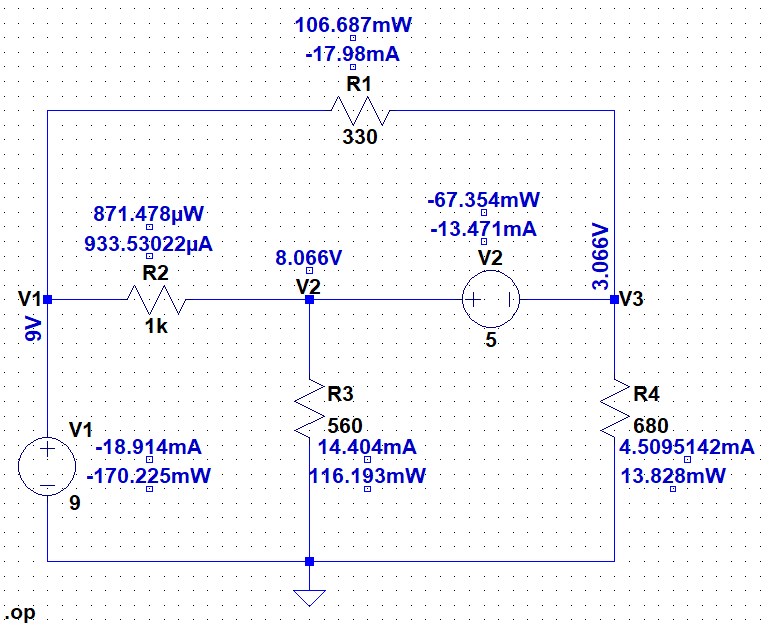
\includegraphics[width=.65\linewidth]{img/sim1}
    \caption{Circuit simulation}
\end{figure}
\subsubsection{Measurements}
\begin{figure}[H]
    \centering
    \begin{tabular}{|c|c|c|c|}
        \hline
        Measurements & Theoretical Value($\si{\volt}$) & Measured Value($\si{\volt}$) & Simulated
        Value($\si{\volt}$)\\\hline
        $V_1$ & 9.000 & 9.120 &9.000 \\\hline
        $V_2$ & 8.066 & 8.160 & 8.066 \\\hline
        $V_3$ & 3.066 & 3.083 &3.066 \\\hline
    \end{tabular}
    \caption{Calculated, measured and theoretical voltage values for each node}
\end{figure}
\begin{figure}[H]
    \centering
    \begin{tabular}{|c|c|c|c|}
        \hline
        Measurements & Theoretical Value($\si{\milli\ampere}$) & Measured
        Value($\si{\milli\ampere}$) & Simulated Value($\si{\milli\ampere}$)\\\hline
        $I_{R1}$ & -17.982 & -17.780 & -17.980\\\hline
        $I_{R2}$ & 0.934 & 0.940 & 0.871\\\hline
        $I_{R3}$ & 14.403 & 14.408& 14.404\\\hline
        $I_{R4}$ & -4.509 & 4.550 & -4.509\\\hline
        $I_{S1}$ & -18.916& -18.240& -18.914\\\hline
        $I_{S2}$ & -13.473 & -14.050& -13.471\\\hline
    \end{tabular}
    \caption{Calculated, measured and theoretical current values}
\end{figure}
\begin{figure}[H]
    \centering
    \begin{tabular}{|c|c|c|c|c|}
        \hline
    Measurements & Theoretical & Measured & Simulated & 
    Absorb(A)/\\
     &  Power (\si{\watt}) &  Power (\si{\watt})  & Power (\si{\watt}) & Supply(S)\\\hline
        $R_1$ & 0.107 & 0.108 & 0.106 &A\\\hline
        $R_2$ & \num{8.724e-4} & \num{8.940e-4}& \num{8.710e-4}&A\\\hline
        $R_3$ & 0.116 & 0.117 & 0.116 &A\\\hline
        $R_4$ & 0.014 & 0.013 & 0.014&A\\\hline
        $V_{S1}$ & -0.170 &-0.164 & -0.170&S\\\hline
        $V_{S2}$ & -0.067 & -0.067 & -0.067&S\\\hline
        & $\sum\textbf{P}=0.001$ & $\sum\textbf{P}=0.002$ & $\sum\textbf{P}=-0.001$ & \\\hline
    \end{tabular}
    \caption{Calculated, measured and theoretical power values for each component}
\end{figure}
\section{Questions}
\textit{\textbf{Which is a node in an electric circuit?}}

A node is a point where two or more components have a common connection. Corresponds to a union
of wires made of conductive material that have an electrical resistance close to 0.\\
\textit{\textbf{What is the nodal voltage?}}

The nodal voltage is that voltage that is in each node since this is different in each one of the
nodes of the analysis.\\
\textit{\textbf{What is called a reference node?}}

The reference node is the one that contains most of the elements connected to it and is chosen to
simplify the system of equations, since this is given a value of 0 volts\\
\textit{\textbf{Describe what the nodal analysis method consists of in the theory of circuits?}}

In the analysis of nodes, an equation is written for each node, provided that the sum of these
currents is equal to zero at any moment, so that a load Q can never be accumulated in a node.
These currents are written in terms of the voltages of each node of the circuit. Thus, in each
relation the current must be given in terms of the tension that is our unknown, by the
conductance.\\
\textit{\textbf{What are the advantages of applying the nodal analysis method?}}

The advantages of using the method of node analysis is that we can calculate the value of the voltages in each one more easily with a system of linear equations.
\section{Conclusions}
{\large Sabrina:}\\
%
\\[2ex]
{\large Salvador:}\\
%
\\[2ex]
{\large Sebastián:}\\
This time we used nodal analysis to determine voltages in each node (except ground), 
in order to do this, we proposed currents in a way that all nodes complied with Kirchhoff's
current law. Then we were able to start our analysis, however, our circuit had the special
case of \textit{supernode}, this was useful because we had an extra equation. In the
end, our mathematical model just had one variable, after factoring and doing some
operations, we had the voltage value of a node, then, using the other expressions, we
finally had our three voltages. Finally, we used this values to determine current and power
values in all components. 
This kind of analysis was easier to do mathematically speaking, because we
didn't had to solve a linear system of equations, nonetheless, we had to manipulate lots
of rational numbers, so we had to do some extra work in order to solve our equation.
At the end, when we compared our theoretical values and the ones we took from measuring the
circuit, all of our values were quite close, at least in magnitude, however, the measured
current value in $R_4$ differed from the theoretical and simulated value in sign, this could be
attributed to a bad connection of the ammeter in the circuit. 
\end{document}
